\section{Méthode de fabrication du capteur}
\label{chap:capteur}
Les capteurs, constitués de la membrane nanoporeuse, des électrodépositions ainsi que des dépôts physiques en phase vapeur d'or (\gls{pvd}) sont 
fabriquées avec plusieurs membranes différentes et selon 2 méthodes :

\subsection{Membranes à disposition}
\begin{table}[H]
    \centering
    \begin{tabular}{|c|c|}
        \hline
        Matériau de la membrane & Épaisseur de la membrane \\
        \hline
        GTTP                    & 6 à 10 $\mu m$           \\
        \hline
        VCTP                    & 6 à 10 $\mu m$           \\
        \hline
        PI25005                 & 25 $\mu m$               \\
        \hline
    \end{tabular}
    \caption{Matériau des membranes disponibles}
    \label{tab:membranes}
\end{table}

\subsection{Dénomination des échantillons}
\begin{table}[H]
    \centering
    \begin{tabular}{|c|c|c|}
        \hline
        Échantillon & Membrane & Méthode d'électrodéposition \\
        \hline
        D06         & GTTP     & A                           \\
        \hline
        D12         & PI25005  & A                           \\
        \hline
        D13         & PI25005  & B                           \\
        \hline
        D14         & VCTP     & A                           \\
        \hline
    \end{tabular}
    \caption{Dénomination des échantillons}
\end{table}

\newpage
\subsection{Méthode A et B}
Les capteurs ont été conçus soit par la méthode A, soit par la méthode B. Ces méthodes sont expliquées et écrites dans les paragraphes qui suivent :
\begin{itemize}
    \item \textbf{Méthode A}
          \begin{figure}[H]
              \centering
              \begin{subfigure}{0.45\textwidth}
                  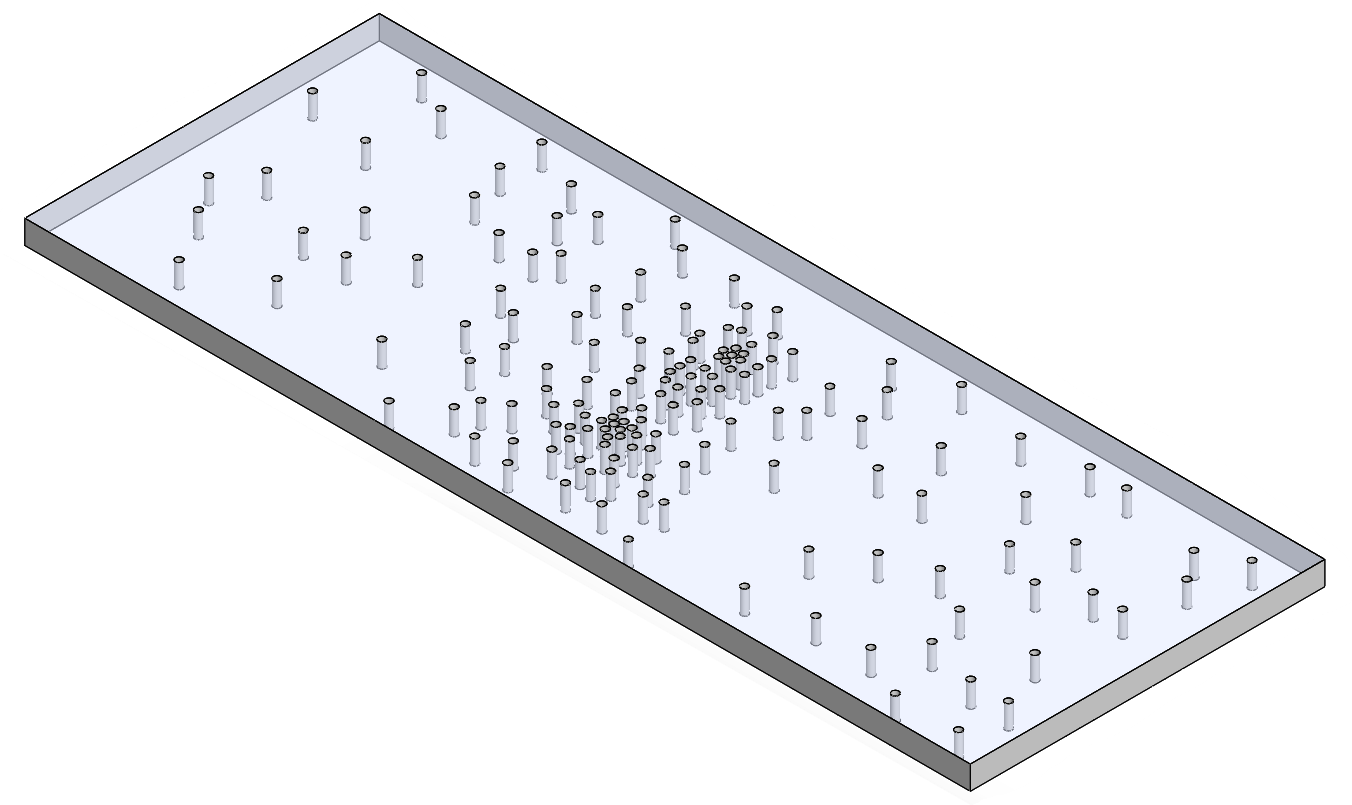
\includegraphics[scale = 0.22]{assets/figures/Membrane_nue.png}
                  \caption{Membrane nanoporeuse}
              \end{subfigure}
              \begin{subfigure}{0.45\textwidth}
                  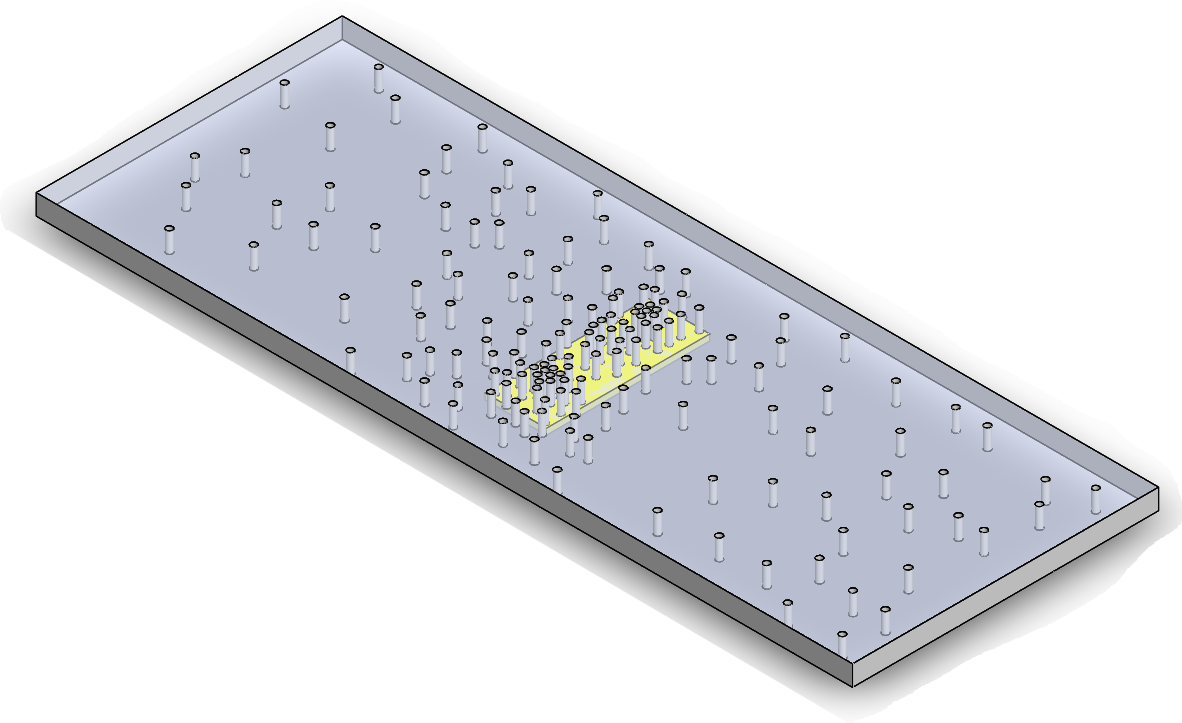
\includegraphics[scale = 0.27]{assets/figures/Court_circuit.png}
                  \caption{Dépôt physique en phase vapeur (PVD) d'or du court-circuit}
              \end{subfigure}
              \newline
              \begin{subfigure}{0.45\textwidth}
                  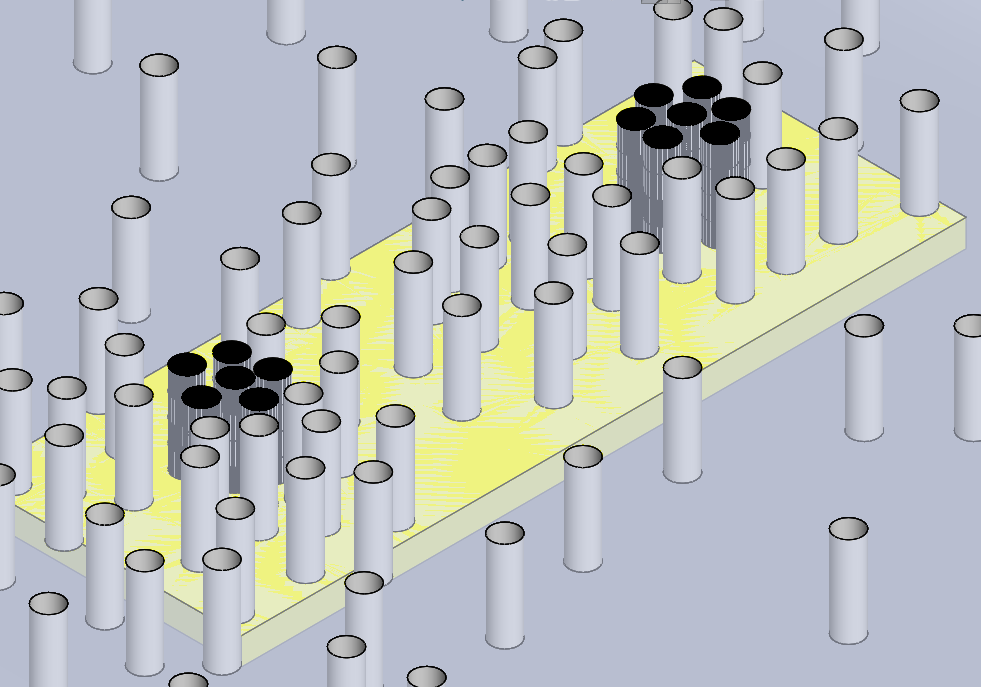
\includegraphics[scale = 0.27]{assets/figures/ED.png}
                  \caption{Électrodépositions effectuées un côté après l'autre}
              \end{subfigure}
              \begin{subfigure}{0.45\textwidth}
                  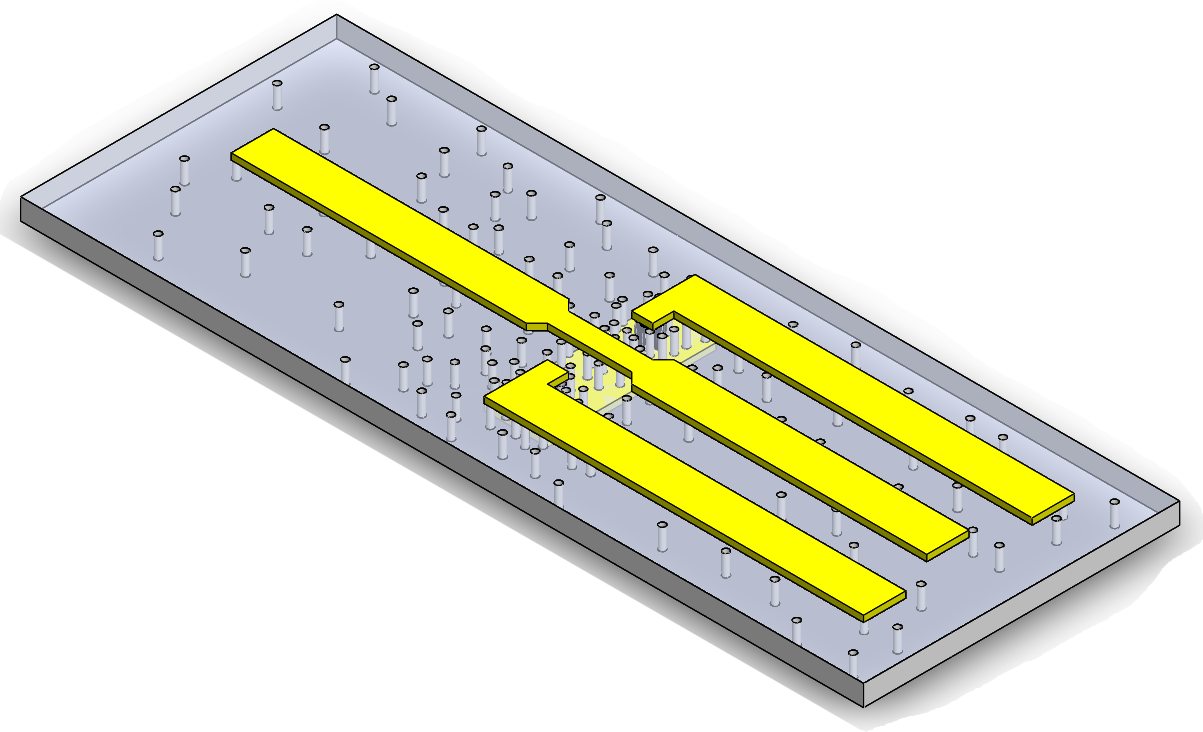
\includegraphics[scale = 0.27]{assets/figures/PVD_L.png}
                  \caption{PVD d'or des branches en L}
              \end{subfigure}
          \end{figure}
          
          \begin{enumerate}[label=(\alph*), wide, labelwidth=!, labelindent = 0pt]
              \item C'est à partir d'une membrane nanoporeuse qu'un capteur est fabriqué. Les différentes membranes sont listées dans le tableau
                    \ref{tab:membranes}. 
              \item Une première \gls{pvd} est effectuée. Pour cette méthodes, de l'or vient se déposer grâce à un masque en forme de bande.
                    Cette couche d'or servira de court-circuit pour le capteur. 
              \item Cette étape concerne les électrodépositions. Une première électrodéposition vient remplir les nanopores de la membrane sur
                    un diamètre défini (nommé diamètre du via). Puis une seconde se fera de l'autre côté de la couche d'or du court-circuit.
              \item La dernière étape de cette méthode consiste à effectuer une \gls{pvd} sur l'autre face de la membrane. Cette \gls{pvd} formera
                    le circuit du themrmocouple complet ainsi que le corps de chauffe (au centre). 
          \end{enumerate}
          
    \item \textbf{Méthode B}
          \begin{figure}[H]
              \hspace{-0.5cm}
              \begin{subfigure}{0.45\textwidth}
                  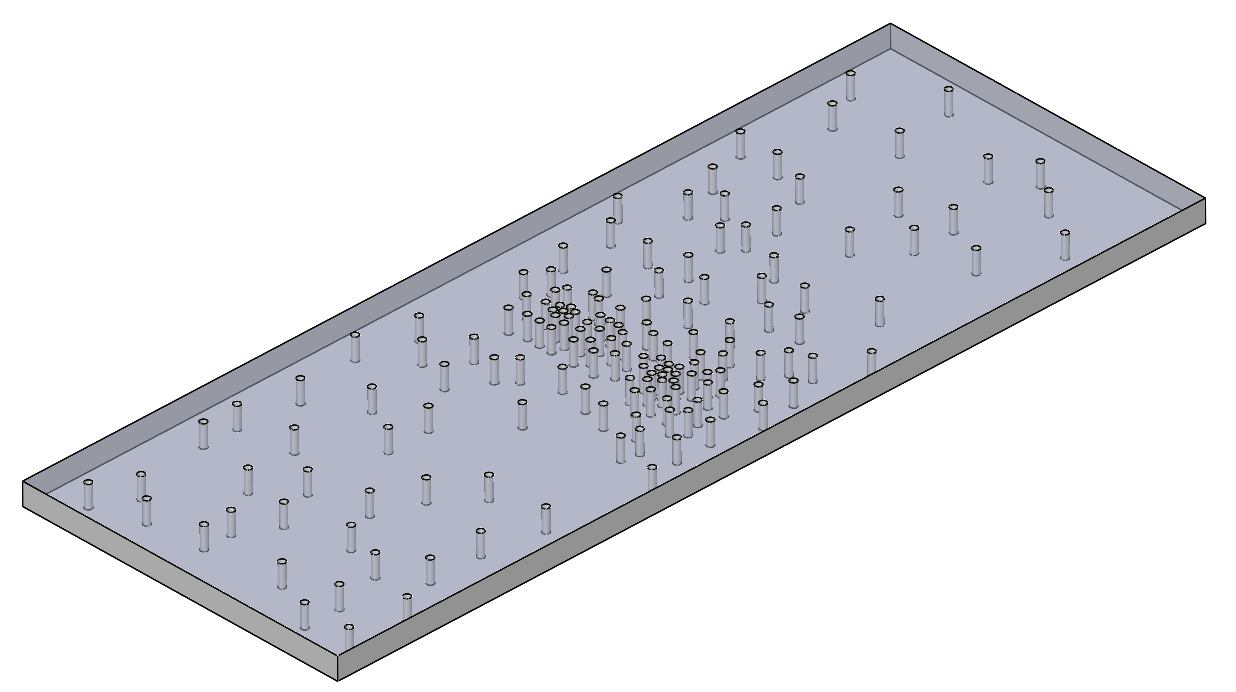
\includegraphics[scale = 0.27]{assets/figures/Membrane_nue_B.png}
                  \caption{Membrane nanoporeuse}
              \end{subfigure}
              \begin{subfigure}{0.45\textwidth}
                  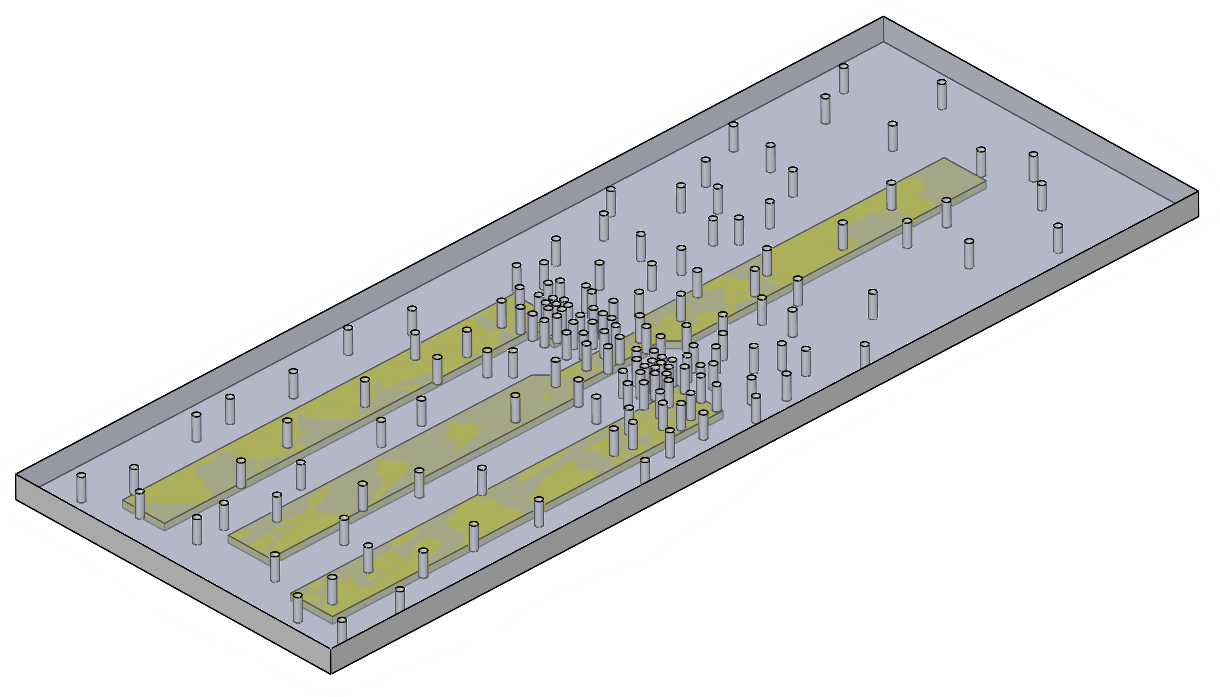
\includegraphics[scale = 0.27]{assets/figures/PVD_L_B.png}
                  \caption{PVD d'or des branches en L}
              \end{subfigure}
              \newline
              \begin{subfigure}{0.45\textwidth}
                  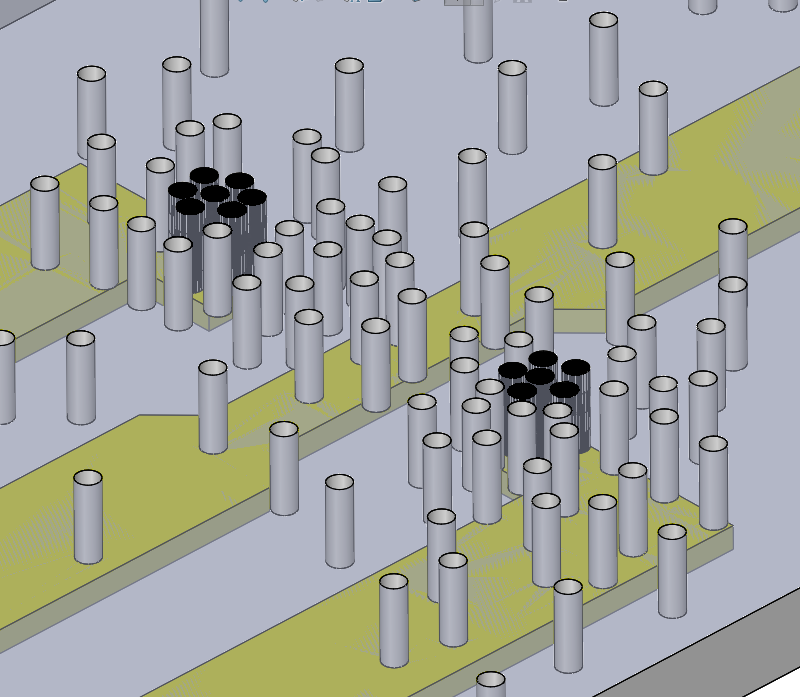
\includegraphics[scale = 0.27]{assets/figures/ED_B.png}
                  \caption{Électrodépositions effectuées une après l'autre}
              \end{subfigure}
              \begin{subfigure}{0.45\textwidth}
                  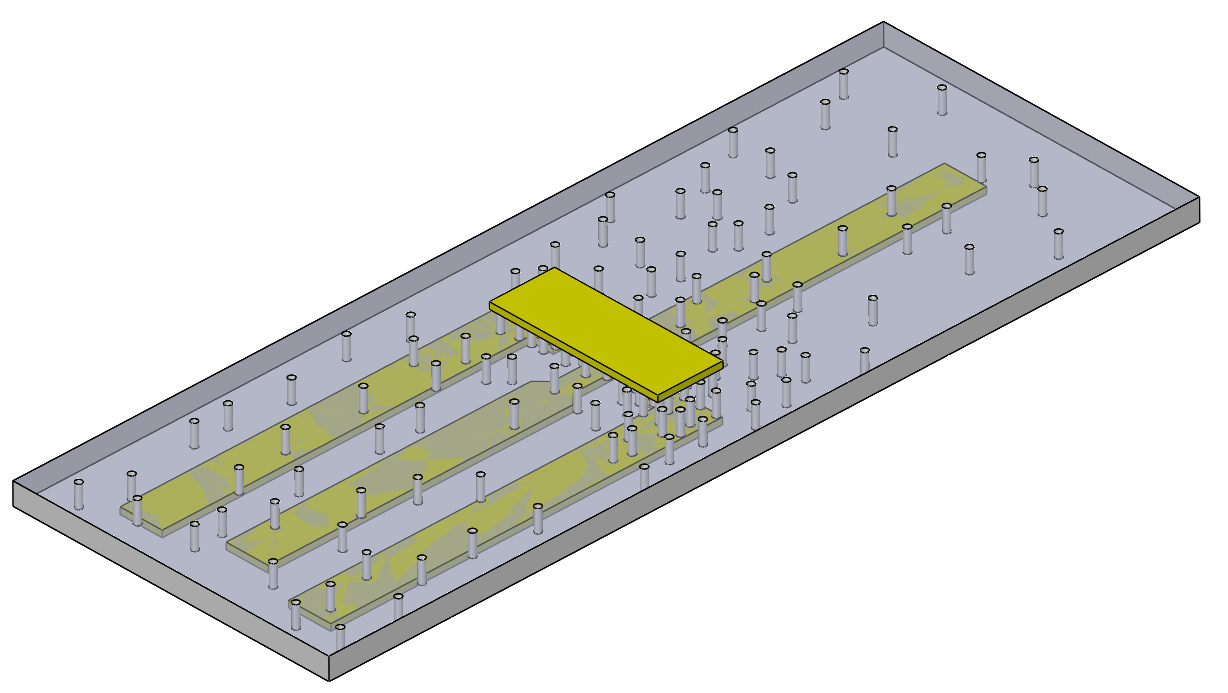
\includegraphics[scale = 0.27]{assets/figures/Court_circuit_B.png}
                  \caption{PVD d'or du court-circuit}
              \end{subfigure}
          \end{figure}
\end{itemize}

\section{Catalogue des solutions du support}
\label{chap:catalogueSol}
Plusieurs systèmes ont été étudiés afin d'incorporer le capteur dans une conception permettant de connecter les membranes et le corps de chauffe
ainsi que d'y attacher un système apportant un flux d'air (imitation de la respiration du patient). Ces différentes solutions seront appeléess
"Support des capteur \gls{capteur}s".

\subsection{Design 1}
\begin{figure}[H]
    \centering
    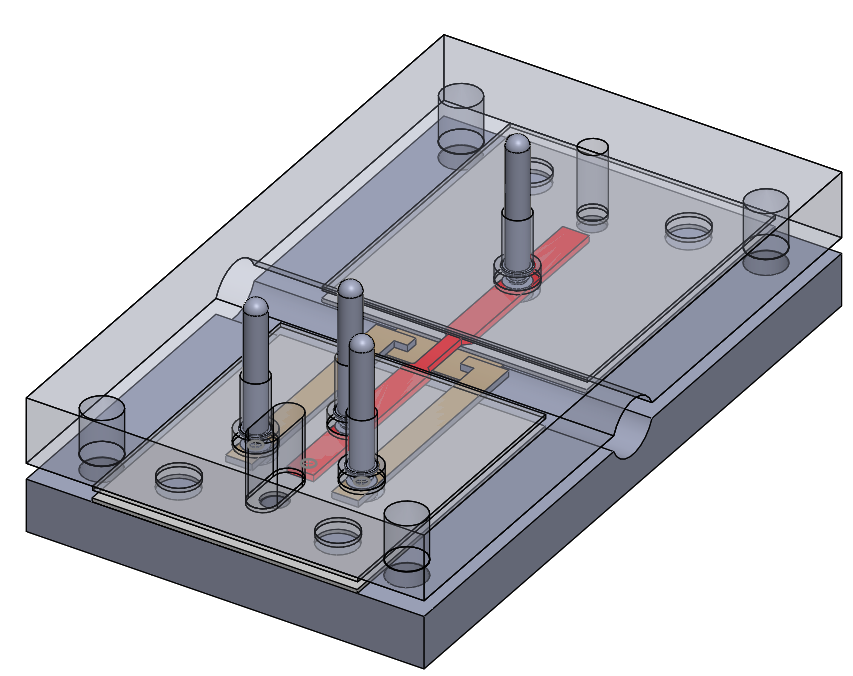
\includegraphics[scale = 0.3]{assets/figures/Design7.png}
    \caption{Design 1}
    \label{fig:design1}
\end{figure}
Ce premier design est le plus basique. Il vient plaquer le capteur entre deux couches presque semblables. Sur une des couches se trouvent des
perçages permettant de tenir des contacts à ressorts (pointes ressorts). Celles-ci viennent s'appuyer d'un côté sur le capteur et
de l'autre, une  connection pourra être faite par des pinces crocodiles ou des soudures. \\
Un joint plat peut venir de part et d'autre du capteur afin d'assurer l'étanchéité du système.\\
Cette solution a le désavantage d'avoir une arrivé d'air scindée en deux. Le placement ainsi que l'étanchéité au niveau de l'entrée
d'air risque d'être mauvaise. \\
Ceci mis de côté, c'est une solution simple, rapide et compacte.

\subsection{Design 2}
Afin d'éviter l'entrée d'air scindée en deux, une solution pourrait être celle représentée ci-dessous :
\begin{figure}[H]
    \centering
    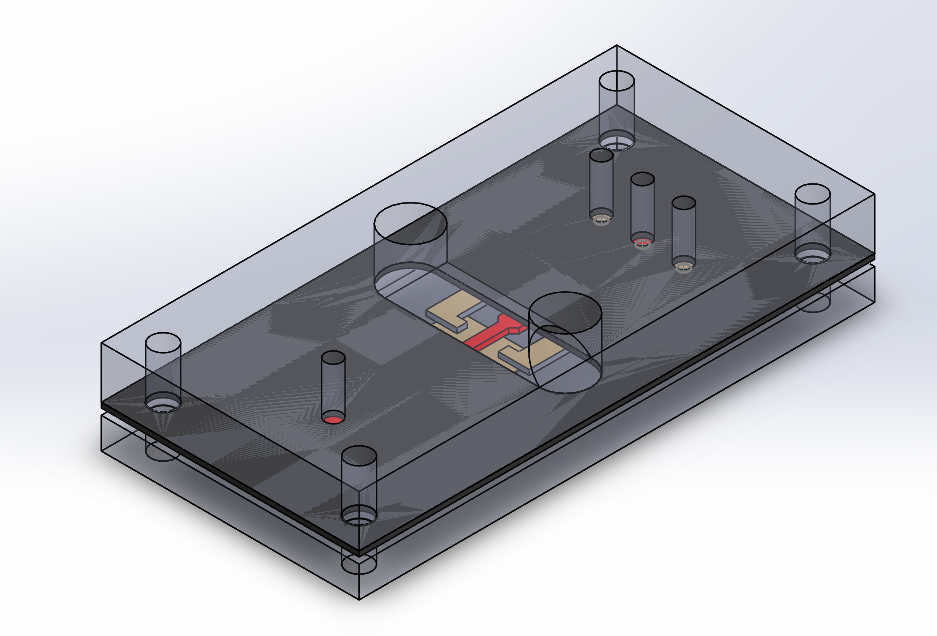
\includegraphics[scale = 0.3]{images/Capteur_design2_caoutch.png}
    \caption{Design 2}
    \label{fig:design2}
\end{figure}
L'arrivée d'air se fait par le haut du système et est dévié par la suite afin d'arriver sur le capteur. Cette solution permet d'avoir une
entrée d'air plus régulière et utilisable que la solution précédente. Cependant, elle ajoute un risque non-négligeable au niveau des turbulences. En effet,
les coudées risquent d'engendrer des turbulences au niveau du flux qui pourraient altérer les résultats.\\
Une particularité à noter est le fait que la membrane se retrouve entièrement plaquée contre une surface contrairement à la solution
précédante où le centre de la membrane (là où est situé le capteur), "flotte" au milieu du flux d'air.

\subsection{Design 3}
Une manière de diminuer les turbulences seraient d'élargir le système afin que les coudées ne se retrouvent pas trop proches de la
membrane.

\begin{figure}[H]
    \centering
    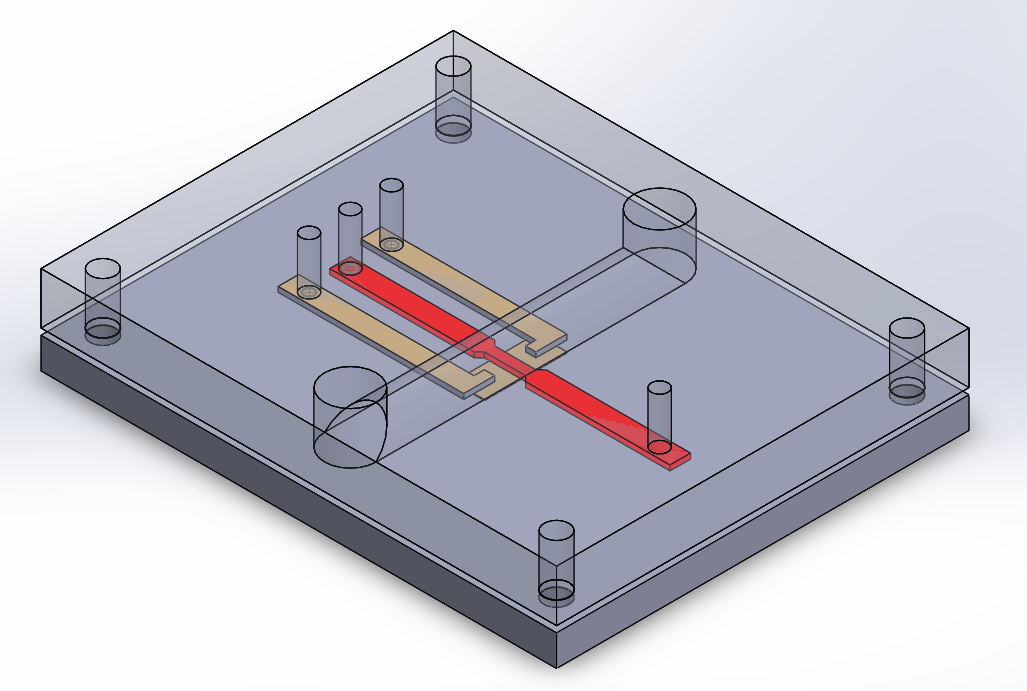
\includegraphics[scale = 0.3]{images/Design4}
    \caption{Design 3}
    \label{fig:design4}
\end{figure}

\begin{comment}
\section{Design 4}
Une autre manière d'éviter ce problème de turbulences et de changer la conception. Ainsi, le capteur pourrait être fabriqué selon la
figure \ref{fig:design6}.

\section{Design 4}%à effacer
\begin{figure}[H]
    \centering
    \includegraphics[scale = 0.5]{images/Design6}
    \caption{}
    \label{fig:design6}
\end{figure}

Cependant cette solution engendre un nombre de pièces plus élevé que les designs précédents. En effet, pour un conception comme celle
de la figure \ref{fig:design6}, 4 pièces seraient nécessaires contre 2 pièces pour les solutions précédentes.\\
Deux pièces viendraient pincer le capteur en sandwich comme montré pour le design 1, figure \ref{fig:design1}, puis, deux autres pièces
viendraient se poser sur les deux longueurs du système afin de permettre de conncter facilement une arrivée d'air.
\end{comment}

\subsection{Design 4}
Finalement, une dernière conception a été imaginée :
\begin{figure}[H]
    \centering
    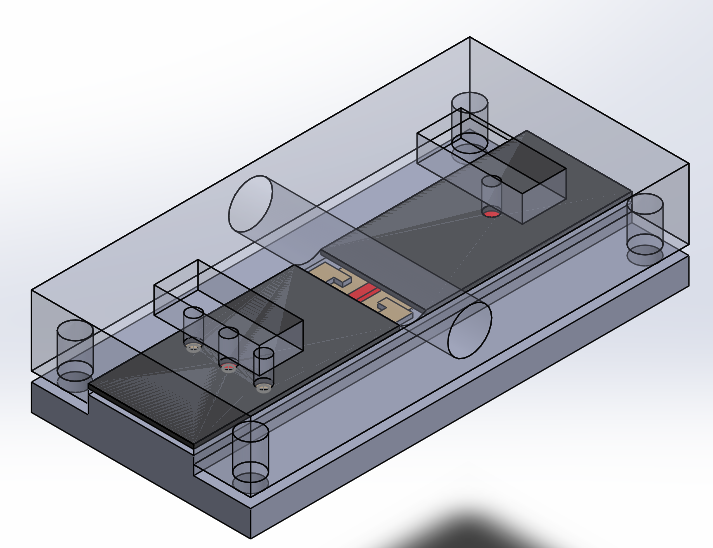
\includegraphics[scale = 0.4]{images/Design5_int_caoutch.png}
    \caption{Design 4}
    \label{fig:design5}
\end{figure}

Cette dernière permettrait de garder une solution à deux pièces seulement et incorporerait une entrée et une sortie d'air facilitée
(non-scindée en deux).\\
La membrane (capteur) posée sur une première pièce légèrement surrélevée. Un joint plat d'échantéité viendrait sur la membrane (en noir
sur la figure). Puis, une seconde pièce viendrait s'appuyer en sandwich contre le joint et le capteur. Cette pièce, sur le dessus, est
percée afin d'amener le flux d'air au niveau du capteur. Des plus petits perçages ainsi que des espaces creusés dans la pièce du dessus
permettent aux pointes ressorts de venir se poser sur la membrane afin d'assurer la connection électrique.\\

Finalement, deux designs ont été retenus. Le Design 1 ainsi que le Design 5. Ces deux designs vont être testés afin de mesurer la
performance d'un capteur recevant un flux d'air depuis le haut et depuis le bas simultanément ainsi qu'un capteur ne recevant un flux
d'air seulement par le haut (car le capteur est plaqué contre une surface).